\section{Preliminary Results}
\label{sec:eval}
\begin{table*}[th]
\caption{Four Original Datasets}
\centering
\begin{tabular}{|c|l|r|r|r|r|} \hline
Dataset	& Description & Records & Dom. Size & Sens. items & Non-Sens. items  \\ \hline \hline
BMS-POS(POS) &Point-of-sale data from a large electronics retailer    &515597 & 1657&1183355 &  2183665\\ \hline
BMS-WebView(WV) &Click-stream data from e-commerce web site  &77512 & 3340& 137605 & 220673  \\ \hline
Retail &  Retail market basket data   & 88162&16470 &340462 & 568114  \\ \hline
Syn & Synthetic data with max record length = 50   & 493193 &5000 &828435 & 1242917 \\ \hline
\end{tabular}
\label{tab:datasets}
\end{table*}

%\begin{figure*}[th]
%\flushleft
%\subfigure[POS]{
%\begin{minipage}[c]{0.23\textwidth}
%\flushleft
%  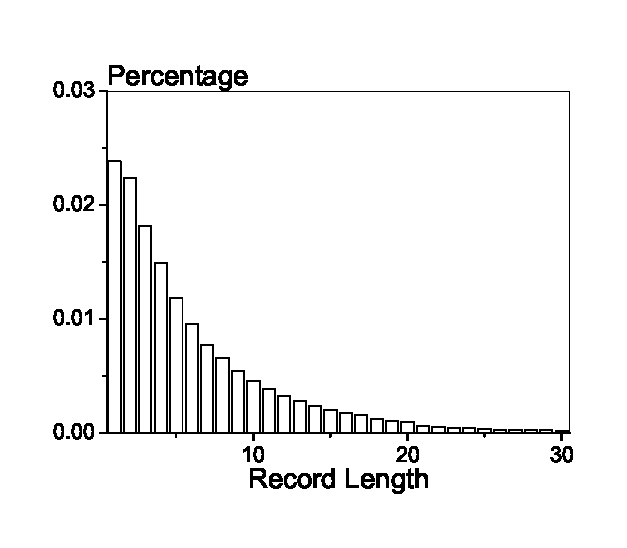
\includegraphics[width=4.5cm]{BMS-POS.eps}
%\end{minipage}%
%}
%\subfigure[WV]{
%\begin{minipage}[c]{0.23\textwidth}
%\flushleft
%  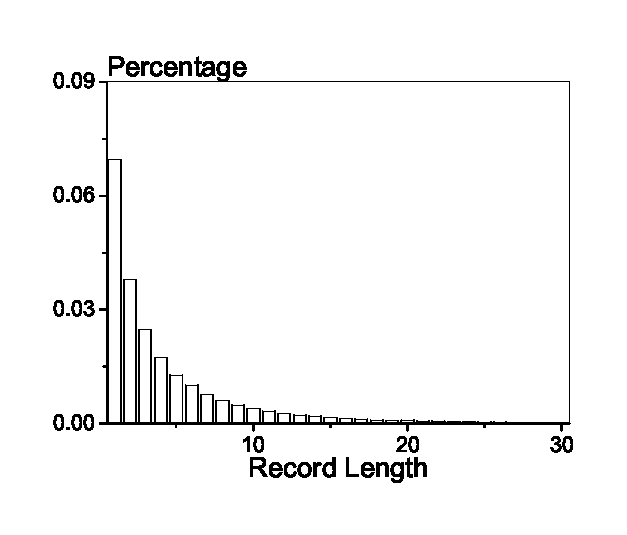
\includegraphics[width=4.5cm]{BMS-WEB.eps}
%\end{minipage}%
%}
%\subfigure[Retail]{
%\begin{minipage}[c]{0.23\textwidth}
%\flushleft
%  \includegraphics[width=4.5cm]{retail.eps}
%\end{minipage}%
%}
%\subfigure[Syn]{
%\begin{minipage}[c]{0.23\textwidth}
%\flushleft
%  \includegraphics[width=4.5cm]{r50w.eps}
%\end{minipage}%
%}
%\caption{Distribution in Record Length of Five Original Datasets}\label{fig:datasets}\shrink
%\end{figure*}


% \begin{figure*}[th]
% \flushleft
% \subfigure[POS]{
% \begin{minipage}[c]{0.23\textwidth}
% \flushleft
%   \includegraphics[width=4.5cm]{itembms.eps}
% \end{minipage}%
% }
% \subfigure[WV]{
% \begin{minipage}[c]{0.23\textwidth}
% \flushleft
%   \includegraphics[width=4.5cm]{itemwv.eps}
% \end{minipage}%
% }
% \subfigure[Retail]{
% \begin{minipage}[c]{0.23\textwidth}
% \flushleft
%   \includegraphics[width=4.5cm]{itemretail.eps}
% \end{minipage}%
% }
% %\subfigure[Syn-1]{
% %\begin{minipage}[c]{0.18\textwidth}
% %\flushleft
% %  \includegraphics[width=4.5cm]{itemr10w.eps}
% %\end{minipage}%
% %}
% \subfigure[Syn]{
% \begin{minipage}[c]{0.23\textwidth}
% \flushleft
%   \includegraphics[width=4.5cm]{itemr50w.eps}
% \end{minipage}%
% }
% \caption{Distribution in Item Frequency of Five Original Datasets}
% \shrink
% \label{fig:datasets2}
% \end{figure*}

%\section{Experimental Results}
%\label{sec:eval}

To evaluate our partial suppression algorithm,
% and understand the effects of
%various parameters in the algorithm,
we conducted a series of experiments on
4 main datasets in Table \ref{tab:datasets}. {\em BMS-POS} and {\em BMS-WebView} are
introduced in \cite{Zheng:2001:RWP:502512.502572} and are commonly used for
data mining. {\em Retail} is the retail market basket data provided by an anonymous
supermarket store \cite{brijs99:retailData}. {\em Syn} is the synthetic data in
which each item is generated with equal probability and the max record length
of 50.
%Figure \ref{fig:datasets}  shows the record length distribution
%of the four datasets.
Since there is no distinction between sensitive and non-sensitive data,
 we randomly designate 40\% of the item types in each dataset as
sensitive items and the rest of the items are non-sensitive.

%We also create another five datasets by setting cutoff to fifty.
%\KZ{Explain how we obtain these datasets. Cite the relevant sources.
%Say how we synthesize the Syn-1 and Syn-2. And say something about cutoff=5
%version of the dataset.}
%\XH{Chao Explained below}

We compare our algorithm with the state-of-the-art global suppression
algorithm (named Global) and generalization algorithm (named TDControl) of
Cao {\em et al.} \cite{Cao:2010:rho}\footnote{The source code of these
algorithms was directly obtained from Cao.} since no other previous work
satisfies our privacy model. We reuse the definition of {\em information loss}
by Cao {\em et al.} \cite{Cao:2010:rho}. In the rest of the section, by {\em
Global} and {\em TDControl}, we mean these two algorithms. Our algorithm has
two variants, \psdist and \psrule which use the two heuristics discussed
previously and optimize for data distribution and rule mining, respectively.
%We also compare the performance of the above
%algorithms with a simple baseline algorithm denoted as {\em Random} which
%randomly picks one unsafe \qid and one item type in this \qid to suppress.

The original datasets take too long to mine association rules.
 To enable the comparison in rule mining, we preprocessed the
original datasets into four additional datasets with the max record length equals 5
, and annotate such datasets with ``cutoff = 5''.

In all experiments, we impose a time limit of
2 hours, and experiments that failed to complete by 2 hours is marked
as ``N/A'' or a zero-height bar in the bar charts.
 %However, both TDControl and global
 %suppression are unavailable in large datasets, thus we cannot make %comparisons in Syn-1 and Syn-2 and Retail where $\rho=0.3$
 %with them.
%reported by Cao \etal \cite{Cao:2010:rho}
%against the same data sets.
%Cao {\em et al.} were very supportive of our work and gave us their code directly.
We run all the experiments on Linux (2.6.34) with an Intel 16-core 2.4GHz CPU
and 8GB RAM. Experiment programs are written in C++ and compiled using GCC
version 4.5.0.

%All experiments effectively use just one core since programs are single
%threaded, except for the experiment in Section \ref{sec:eval:performance}
%where we demonstrate the result of a multi-threaded version of
%our algorithm in Table \ref{tab:timeresult}.

%We have 3 real data sets and 2 synthetic data sets in total.
%Prepare the data in large, medium and small sizes. Compare our algos
%with the competing algorithms in rho-uncertainty paper against all
%data sets. Record the time, number of items suppressed, relative entropy,
%and number of rules learned in each of the experiments.
%
%Scaling test: divide the 3 real data sets into 10 parts, and run
%our algos on 10\%, 20\%, 30\%, ... of the whole data sets and plot
%diagram of time and quality of solution.
%
%Add more??

%\begin{itemize}
%\item Explain the implementation of the three variants of our partial algorithm
%(i.e., Partial(R), Partial(L) and Partial(ALL)).
%Explain any implementation details that were not covered by
%the algorithm section. Say how we pick the different params for the algorithm
%and any heuristics options, e.g., random, long record first, long qids first,
%etc.
%\item Explain the implementation details of two of our competitors, TDControl
%and global suppression. How we obtained the code.
%Anything special about the implementation that is different from
%the $\rho$-uncertainty paper.
%
%\item Compare the results in information loss (explain the different metric
%in information loss between us and TDControl), symmetric relative entropy
%(explain what it is and cite) and number of association rules mined. Explain
%the cutoff time of 2 hours in our experiments. That is if the experiment
%exceeds 2 hours, we kill the program. Discuss how we outperform the other
%competitors and why.
%
%\item Compare our results with the optimal solution on small datasets. Explain
%how we get the small dataset first. I think we wanna say it's a subset of
%the cutoff=5 version. Is that true? Discuss why our results are not far
%from the optimal.
%
%\item Discuss the how the iterative algorithm fixes the unsafe qids and how
%bad is the regression. How many iterations are there for a typical dataset?
%How long does each iteration take?
%
%\item Show the scalability results of our algorithms on 3 datasets.
%
%\item Discuss the effects of varying the buffer size $b$ on execution time
%and information losses.
%
%\item Discuss the effects of varying estimated cost bound on the number
%of partitions created, execution time, and info loss.
%
%\item Discuss the effects of varying long record bound on execution time
%and information losses.
%
%\item Discuss the effects of varying long record processing (1000 each time)
%on execution time and information losses.
%\KZ{Do we still have these results?}
%
%\item Discuss the effects of preprocessing (cutting long records).
%\KZ{Do we still have these results?}
%
%\item Give a little summary to this section.
%\end{itemize}
%
%\KZ{END OF OUTLINE.}

%We used 5 datasets in our experiment. BMS-POS and
%BMS-WebView are introduced in \cite{Zheng:2001:RWP:502512.502572} and are
%commonly used for data mining. Retail is the retail market basket data
%provided by an anonymous supermarket store \cite{brijs99:retailData}.
%Syn-1 and Syn-2 are artificially synthetic data by us according to the
%standard that items are made even distributed.
%Figure \ref{fig:datasets} shows the general distribution of the five
% datasets. We see that long records account for only a small portion among
%  all datasets.
%  and the distribution of Retail has a outstanding ascending curve
%  from record length one to record length four, then goes down as others do
%  in longer record length. While Retail dataset also contains more
%  percentage of records with the same small length compared with
%   other four datasets.
  %Although some anomalies exists in retail, it remains the distribution when the record length comes to four.
%  It's reasonable to be explained that
%  customers usually buy more than one goods when they go shopping.
%  To make some comparison possible, like comparing the rules mined
%  from results of all algorithms, we cut off original datasets into
%  other five corresponding datasets which contain only records no more than
%  five items, like Retail(cutoff=5) or Syn-1(cutoff=5). We also create
%  another five datasets by setting cutoff to fifty.


In what follows, we first evaluate the effects of our divide-and-conquer
strategy and then we show the result of the data utility. Unless otherwise
noted, we use the following default parameters: $b_{max} = 10^6$ ,
$t_{max}=500$, $\rho =0.7$.
 %In addition, we set records whose length larger than 12 as
%long records.
%%and we set 1000 as our local optimal buffer.
%See Section
%\ref{algo:impmentation}.
%$t_{max}$ = 400 secs\PC{New paramater},
 %$\lmin=12$, $\dnum = 1000$.
% Divide-and-conquer parameters
% $\alpha$, $\beta$, $\gamma$ in Equation (\ref{eq:costfunc}) are learned to
%be 1.71E-8, 1.49E-5 and 3.06 ,
%respectively. \PC{Parameter redefinition}

%Apart from these above parameters, we compare the performance of
%three partial suppression policies (\PartialR, \PartialL and \PartialALL).

  %in order to prove that deleting only sensitive items is the best choice.
%The function
%of these three heuristics is specifically introduced before and we also tested them separately.
%Although some heuristics work in
%some data sets, the general performance of these three methods are almost the same.
% Given that randomness is the most
% simpleness way to solve this problem, we choose the method of randomly picking eventually to present.
%
 %\subsection{Competitors}
%\KZ{Move this subsection to the beginning of the section where we
%talked about Cao's implementation.}

 %Here we introduce the latest work of the global suppression and TDControl of  Cao {\em et al.} \cite{Cao:2010:rho}
 % as the competitors, because they represents a standard global suppression and generalization method based on the greedy algorithm.
 %We also set a cutoff time of 2 hours to prevent the program from running for too long. However,both TDControl and global
 %suppression are unavailable in large datasets,thus we cannot make comparisons in Syn-1 and Syn-2 and Retail where $\rho=0.3$
 %with them.

\subsection{Effects of Divide-and-Conquer}\label{sec:eval:effect}
In this section, we analyze the effectiveness of the divide and conquer
strategy on the quality of solution (in terms of information loss) and time
performance using the dataset {\em Retail}.
%parameters for optimization defined in our algorithm help to ameliorate the time performance by the largest extent but remain the quality of the suppressed datasets.
%We have 4 different parameters including partial suppression policies
%
%\subsubsection{Partial Suppression Strategies}\label{sec:eval:partialsuppression}
%The following experiments illustrate the result of different suppression
%strategies. Figure \ref{sec:eval:infoloss} suggests that $Mine$ outperforms
%the other two different strategies in information loss and association rule
%mining (See Table \ref{tab:rules2}) but doesn't do as well in relative
%entropy. $Dist$ outperforms the other two strategies in retaining the data
%distribution. The log function we take on the y-axis indicates that relative
%entropy of $Dist$ is much better than peers. Although it doesn't perform well
%in information loss, such a disadvantage doesn't outweigh its advantage.
%Since the occurrence of each item in the dataset remains almost the same and
%the probability of each item can be precisely estimated. Time performances of
%the three approaches are in the same range. We therefore conclude that the
%performances of our two heuristics are in our expectations and such processed
%result can be highly useful for downstream applications.
%
%\begin{figure}[th]
%\centering
%  \flushleft
%\subfigure[ $\rho=0.7$]{\label{fig:partialrelative}
%\hspace{-5mm}
%\begin{minipage}[c]{0.22\textwidth}
%\flushleft
%  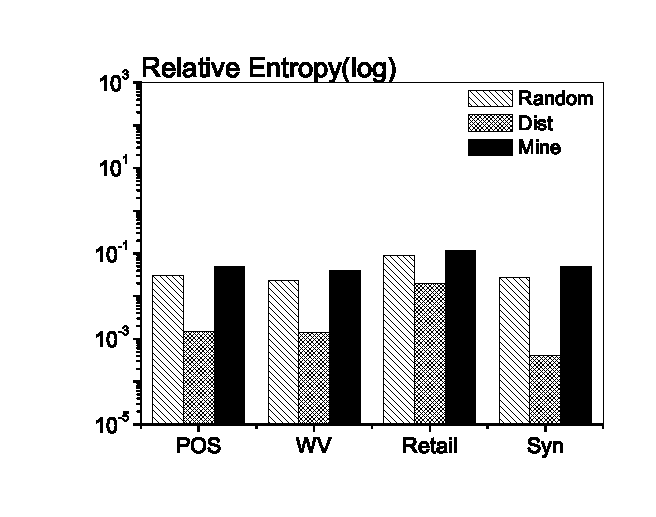
\includegraphics[width=4.9cm]{relative7ours.eps}
%\end{minipage}%
%}
%\subfigure[ $\rho=0.7$]{
%\hspace{3mm}
%\begin{minipage}[c]{0.20\textwidth}
%\flushleft
%  \includegraphics[width=4.5cm]{partialtime.eps}
%\end{minipage}%
%}
%\caption{Comparison among Partial Suppression Strategies}
%\label{fig:partial}
%%\textit{Partial(R)} suppresses sensitive only, \textit{Partial(L)} suppresses items on left side of a inference, and \textit{Partial(ALL)} suppresses items on both sides of a inference.}\label{fig:fft}
%\end{figure}

%\subsubsection{Variation of $t_{max}$}\label{sec:eval:timebound}
% since $Retail$ is the most
%time-consuming datasets which can terminate within an acceptable time without DnC strategy.
%The value of $t_{max}$ determines the size of a partition in DnC. Smaller
%$t_{max}$ can give rise to more partitions.
%Here, we
%evaluate how partitioning helps with time performance and
%its possible effects on suppression quality.

Figure \ref{fig:timebound-a} shows the relationship between the number of
partitions and the information loss. The line of \psdist is flat and \psrule
shows only a slight ascend, which indicates that reducing $t_{max}$ and hence
increasing the number of partitions doesn't sacrifice the quality of the
solution. Furthermore, Figure \ref{fig:timebound-b} shows that time cost
decreases dramatically with the increase of partitions which highlights the
benefits of D\&C. The main reason for the speed-up is that the time
complexity is exponential to the scale of the partition.
%, the cost of enumerating \qids which is the most
%time-consuming part in our algorithm.
Another reason is the D\&C well exposes the parallelism for parallel computation.


%This can be explained by Equation (\ref{eq:costfunc}).
%As Figure \ref{fig:scale:b} shows,
%the time cost for \PartialR on Retail is a slow exponential function, say
%$\epsilon^{|T|}$ where $\epsilon$ is small. Now, if decreasing $t_{max}$ causes
%a split of data into equal halves. The expected time cost will be
%$2\epsilon^{\frac{|T|}{2}}$. This rough estimation clearly gives rise to
%an exponential speed up.


%Figure \ref{fig:timebound} shows that the time performance increases
%exponentially with the increase of $t_{max}$.However, the quality of our result almost remains the same, which indicates that
%partition is a reasonable method which can be applied to our algorithm.
%The line tends to be plain when $t_{max}$ becomes larger,
%because the expected time is less than $t_{max}$,
% suggesting that no partitions will be executed.

%timebound
\begin{figure}[th]
\flushleft
\subfigure[Information Loss]{
\label{fig:timebound-a}
\hspace{-4mm}
\begin{minipage}[c]{0.23\textwidth}
\flushleft
  \includegraphics[width=4.7cm]{timeloss.eps}
\end{minipage}%
}
\subfigure[Time Performance]{
\label{fig:timebound-b}
\begin{minipage}[c]{0.23\textwidth}
\flushleft
  \includegraphics[width=4.7cm]{timetime2.eps}
\end{minipage}%
}
\caption{Effects of Partition Size on Information Loss and Running Time 
($\rho = 0.7$)}\label{fig:timebound}
\end{figure}
%\PC{The figure use 1/t is not very elegant. see figure 2(a). If you guys think that's OK. I will repaint the pic.}
\subsection{Data Utility}\label{sec:eval:datautility}
In this section we compare the utility of the anonymized data produced by
our algorithm, global suppression and TDControl in terms of information loss,
data distribution, and association rule mining.

%\subsubsection{Information Loss}\label{sec:eval:infoloss}
%
%\begin{figure}[th]
%\flushleft
%\subfigure[ $\rho=0.3$]{\label{fig:loss-a}
%\hspace{-4mm}
%\begin{minipage}[c]{0.23\textwidth}
%\flushleft
%  \includegraphics[width=4.7cm]{loss3.eps}
%\end{minipage}%
%}
%\subfigure[ $\rho=0.7$]{\label{fig:loss-b}
%\begin{minipage}[c]{0.23\textwidth}
%\flushleft
%  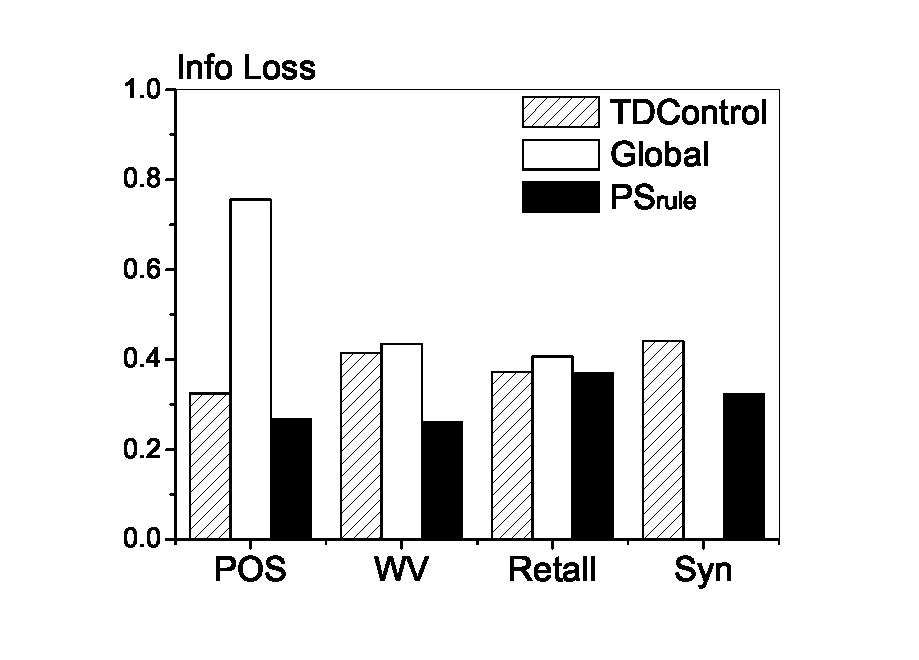
\includegraphics[width=4.7cm]{loss7.eps}
%\end{minipage}%
%}
%\caption{Comparative Results in Information Loss}\label{fig:loss}
%\end{figure}

\begin{figure}[th]
\flushleft
\subfigure[Info Loss]{\label{fig:loss7}
\hspace{-4mm}
\begin{minipage}[c]{0.23\textwidth}
\flushleft
  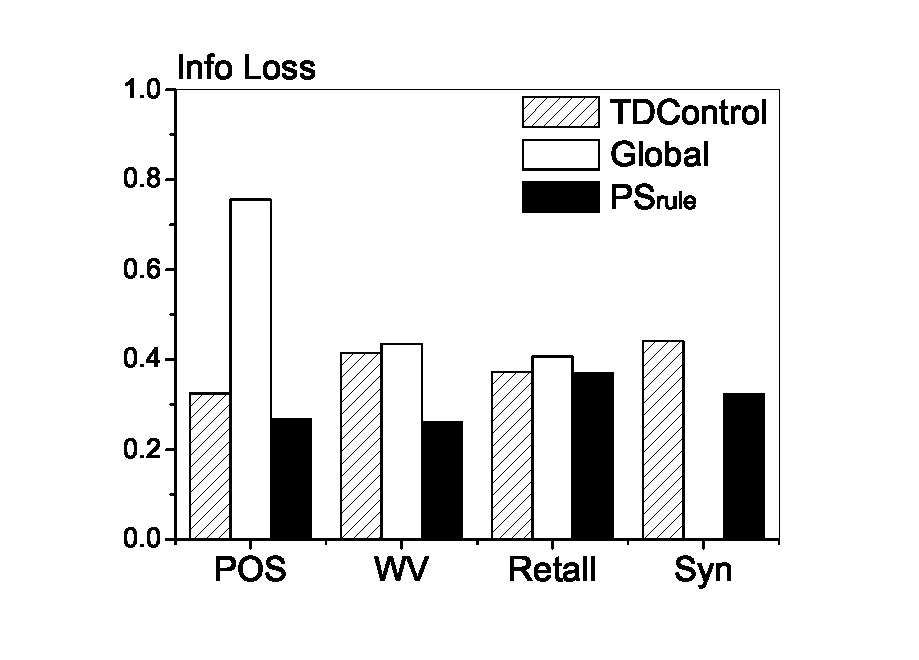
\includegraphics[width=5cm]{loss7.eps}
\end{minipage}%
}
\subfigure[Relative Entropy]{\label{fig:rela7}
\begin{minipage}[c]{0.23\textwidth}
\flushleft
  \includegraphics[width=5cm]{rela7.eps}
\end{minipage}%
}
\caption{Comparative Results on Data Utility}\label{fig:loss}
\end{figure}


%The first comparison is based on information loss (Definition
% \ref{def:infoloss}).
%To enable comparison with TDControl which generalizes items in addition to
%suppressions, we adopt the generalized form of information loss metric introduced
% by Cao \etal \cite{Cao:2010:rho}, which is identical to Definition \ref{def:infoloss} when
% only suppression is performed.

%loss metric introduced \cite{Cao:2010:rho}:
%%\[ IL(T,T^\prime)=\frac{\sum_{e\in D}sup(e)\cdot Loss(e)}{\sum_{e\in D}sup(e)}\]
%%where
%%\[ Loss(e)=\begin{cases}
%%  \frac{leaves(n)}{Dom(n)}, & \text{if item $e$ is generalized to node $n\in\mathcal{H}$}\\
%%  1,                          & \text{if item $e$ is suppressed.} \\
%%\end{cases} \]
%%Note this definition is the same as Definition \ref{def:infoloss} if there is
%%only suppression. \XH{Change to: We use the generalized form of information
%loss metric introduced by Cao \etal \cite{Cao:2010:rho} to compare with
%TDControl, which is identical to Definition \ref{def:infoloss} when
%suppression is used.
% }

From Figure \ref{fig:loss7},
%we find that $Dist$ performs similarly  with Global and $Random$ performs
%similarly with TDControl.
we conclude that \psrule is uniformly better among the other two techniques.
It suppresses only about 26\% items in POS and WV and about 35\% items in
{\em Retail}, while the other four techniques incur on average 10\% more losses
than \psrule and up to 75\% losses in the worst case.
%We notice that $Dist$
%performs worse than  $Random$ even it tries to minimize the information loss
%at each iteration. The reason is that it also tries to retain the data
%distribution.


Figure \ref{fig:rela7} shows that \psdist outperforms the peers
 as its output has the highest resemblance
to the original datasets. On the contrary, TDControl is the worst performer
since generalization algorithm creates a lot of new items while suppressing
too many item types globally. Since the symmetric relative entropy of \psdist
is very small, we use log scale on the y-axis to highlight the differences.
%Therefore, although the height difference is not huge, the real difference is
%tremendous with a difference of even two or three orders.
%We only use \psdist as our competitor since \psdist is supposed to
%remain the data distribution.
%However, the other two partial strategies also outperform global and TDControl in retaining data distribution.
%\PC{Do we need to mention it?}


Table \ref{tab:rules2} gives the results for the association rules mining.
The ``Original'' row records the number of rules that can be mined from the
original data. ``Spurious \%'' denotes the percentage of the inferred rules
that are extraneous. Both TDControl and Global are outperformed by our method
in this category, with negligible number of original rules remaining after
anonymization. Conversely, both of the partial suppression algorithms manage
to retain most of the rules, with only a fraction (about 10\%) of which are
spurious. Specifically, \psrule performs the best. We argue that for
downstream rule mining applications, results from Global are almost useless
even though it introduces no extra rules. On the other hand, generalization
is only useful if the generalization hierarchy is recognized by the data
user.
% Although $Random$ outperforms $Mine$
%in two datasets in spurious probability, the uncertainty of the performance  cannot
%guarantee the practicability.
%Furthermore, $Mine$ retains the most
%rules in all dataset. Checking the anonymized datasets, we find that $Mine$ keeps
%most of the items  but suppresses more than half for some items. In other words,
%$Mine$ maintains the support of many items and retains the rules mined from them.


%Note that these new, more general rules from the result of TDControl can be
%``specialized'' into rules of original level in the generalization hierarchy.
%For example, we can specialize a rule \{dairy product $\rightarrow$ grains\}
%into
%\{milk $\rightarrow$ wheat\},
%\{milk $\rightarrow$ rice\},
%\{yogurt $\rightarrow$ wheat\},
%\{yogurt $\rightarrow$ rice\}, etc.
%%However, the newly generated rules only account for a small part
%%in the rules mined from result of
%%\PartialR and what matters more is that remained rules still occupy a
%%large portion compared with the original rules based on the experiment
%%result in Table \ref{tab:rules}. New rules may also be generated by
%%generalization, since the domain of the generalized dataset
%%is different from the original one. A reasonable way
%%to transfer the newly generated rules by generalization is to
%%replace the newly generalized item with specific items which are its
%%descendants. For example, if there exists a generalized rule
%%$\{1\ 2\ 3\rightarrow \alpha\}$ where $1=\{b\ c\}, 2=\{d\},
%%3=\{e\ f\}$, we can transfer this rule into four different rules such
%%as $\{b\ d\ e\rightarrow \alpha\}$,  $\{b\ d\ f\rightarrow \alpha\}$,
%%$\{c\ d\ e\rightarrow \alpha\}$, $\{c\ d\ f\rightarrow \alpha\}$.
%%Through this strategy, we can now compare rules mined from the result
%%of TDControl and \PartialR in the same level of item domain.
%Take BMS-POS(cutoff = 5) for an example. 6 generalized rules are
%mined from TDControl result. After specializing we get
%278852 possible rules with only 2 of them in the original rules!
%
% Yet, we will see how this heuristic works in retaining the data
%distribution in Section \ref{sec:eval:datadistribution}
%
%
%Note that Global and TDControl failed to complete in some datasets.
%%This confirms that our alogrithm causes less information losses than peers.
%This confirms that our algorithm is more practical than peers.
%indicating that our algorithm has a
%strong flexibility in $\rho$.
%
%\subsubsection{Data Distribution}\label{sec:eval:datadistribution}
%
%\begin{figure}[th]
%\flushleft
%\subfigure[ $\rho=0.3$]{
%\hspace{-4mm}
%\begin{minipage}[c]{0.23\textwidth}
%\flushleft
%  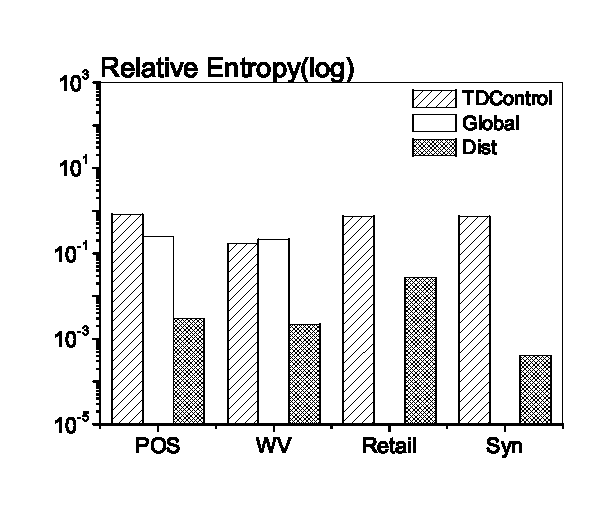
\includegraphics[width=4.5cm]{relative3.eps}
%\end{minipage}%
%}
%\subfigure[ $\rho=0.7$]{
%\begin{minipage}[c]{0.23\textwidth}
%\flushleft
%  \includegraphics[width=4.5cm]{relative7.eps}
%\end{minipage}%
%}
%\caption{Comparative Results in Symmetric Relative Entropy}
%\label{fig:entropy}
%\end{figure}
%
%To determine the similarity between the item frequency distribution
%of original data and that of the anonymized data,
%we use the symmetric relative entropy between the two distributions.
%The ordinary relative entropy
%\cite{Lin91divergencemeasures} which is also called Kullback-Leibler
%divergence is defined as follows.
%\begin{equation} \label{eq:relative}
%\mathcal{R}(H_1||H_2)=\sum_{i=1}^{n}H_1(i)\cdot log(H_1(i)/H_2(i))
%\end{equation}
%where $H_1$ and $H_2$ are two histograms and each $H_1(i)$ and $H_2(i)$ represent the height of the corresponding bar in $H_1$ and $H_2$ respectively.
%To prevent zero denominators, we modified (\ref{eq:relative})
%to a symmetric relative entropy \cite{Fisher:2008:DSF} defined as
%\[\mathcal{S}(H_1||H_2)=\frac{1}{2}\mathcal R( H_1||H_1 \oplus H_2)+\frac{1}{2}\mathcal R( H_2||H_1 \oplus H_2)\]
%where  $H_1 \oplus H_2$ represents the union of the $H_1$ and $H_2$.
%
%Figure \ref{fig:entropy} shows that $Dist$ outperforms the peers
% as its output has the highest resemblance
%to the original datasets.
%On the contrary, TDControl is the worst performer
%since generalization algorithm creates a lot of new items while
%suppressing too many item types globally.
%Since the symmetric relative entropy of $Dist$ is very small, we use log function
%on the y-axis to make the result visible. Therefore, although the height difference
%is not huge, the real difference is tremendous with a difference of even two or three orders.
%We only use $Dist$ as our competitor since $Dist$ is supposed to remain the data distribution.
%However, the other two partial strategies also outperform global and TDControl in retaining data distribution.
%The result is shown in figure \ref{fig:partialrelative}.
%Results of global suppression are five times more than
%those of \PartialR on average,
%despite its relatively higher similarity
%than results of TDControl.

%  The anomaly in WV when {$\rho$} is 0.3 dues to the uncertainty of global suppression method. Figure \ref{fig:entropy}
%illustrates that relative entropy of partial(R) is five times less than both TDControl and global suppression, indicating that the
%remaining distribution is much more similar with the original distribution
%than TDControl and global suppression is.
%
%\subsubsection{Association Rules Mining}\label{sec:eval:rulemining}
%The most common criticism of partial suppression is that it
%changes the support of good rules in the data and introduces spurious
%rules in rule mining. In this experiment, we test the algorithms on
%data sets with the max record length=5(cutoff=5), and check the rules mined from the anonymized data
%with support equals to 0.05\% and confidence equals to 70\%. Mining rules from the original datasets with many
%long records is prohibitive due to large memory requirements.
%
%Table \ref{tab:rules2} gives the results. The ``Original'' row records the
%number of rules that can be mined from the original data. ``Spurious \%''
%denotes the percentage of the inferred rules that are extraneous.
%Both TDControl and Global perform badly in this category, with
%negligible number of original rules remaining after anonymization.
%Conversely, all of of the partial
%suppression algorithms manage to retain most of the rules, with only a
%fraction (about 10\%) of which are spurious. Specifically, $Mine$ performs
%the best among partial algorithms. Although $Random$ outperforms $Mine$
%in two datasets in spurious probability, the uncertainty of the performance  cannot
%guarantee the practicability. Furthermore, $Mine$ retains the most
%rules in all dataset. Checking the anonymized datasets, we find that $Mine$ keeps
%most of the items  but suppresses more than half for some items. In other words,
%$Mine$ maintains the support of many items and retains the rules mined from them.
%We argue that for downstream
%rule mining applications, results from Global are almost
%useless even though it introduces no extra rules. On the other hand, TDControl
%is only useful if the generalization hierarchy is recognized by the data user.
%Note that these new, more general rules from the result of TDControl can be
%``specialized'' into rules of original level in the generalization hierarchy.
%For example, we can specialize a rule \{dairy product $\rightarrow$ grains\}
%into
%\{milk $\rightarrow$ wheat\},
%\{milk $\rightarrow$ rice\},
%\{yogurt $\rightarrow$ wheat\},
%\{yogurt $\rightarrow$ rice\}, etc.
%%However, the newly generated rules only account for a small part
%%in the rules mined from result of
%%\PartialR and what matters more is that remained rules still occupy a
%%large portion compared with the original rules based on the experiment
%%result in Table \ref{tab:rules}. New rules may also be generated by
%%generalization, since the domain of the generalized dataset
%%is different from the original one. A reasonable way
%%to transfer the newly generated rules by generalization is to
%%replace the newly generalized item with specific items which are its
%%descendants. For example, if there exists a generalized rule
%%$\{1\ 2\ 3\rightarrow \alpha\}$ where $1=\{b\ c\}, 2=\{d\},
%%3=\{e\ f\}$, we can transfer this rule into four different rules such
%%as $\{b\ d\ e\rightarrow \alpha\}$,  $\{b\ d\ f\rightarrow \alpha\}$,
%%$\{c\ d\ e\rightarrow \alpha\}$, $\{c\ d\ f\rightarrow \alpha\}$.
%%Through this strategy, we can now compare rules mined from the result
%%of TDControl and \PartialR in the same level of item domain.
%Take BMS-POS(cutoff = 5) for an example. 6 generalized rules are
%mined from TDControl result. After specializing we get
%278852 possible rules with only 2 of them in the original rules!
% So there are 438051 spurious rules!
% This reflects that the support of rules become higher
% after items being generalized, which leads to the fact that
% the newly generated rules is confirmed to exist in original rules only
% when support is set to 1, but meaningless when support is higher.Another
% thing is if data users don't agree on the generalized hierarchy,
% generalized rules are also meaningless.
%
%%table for rules (sup=5 rho=0.7)
%\begin{table}[th]
%\caption{Association Rules Mined with Support $5$ ($\rho=0.7$)}
%\centering
%\begin{tabular}{|l|r|r|r|}
%  \hline
%  % after \\: \hline or \cline{col1-col2} \cline{col3-col4} ...
%   & POS & WV  & Retail \\
% & (cutoff = 5) &(cutoff = 5) & (cutoff = 5) \\\hline \hline
% Original & 4457 & 600 & 674 \\\hline
%  TDControl& 36 & 58 & N/A \\
% (Spurious \%) & (100\%) & (100\%) & N/A \\\hline
%Global & 5 & 98 & 87\\
%(Spurious \%) & (0\%) & (0\%) & (0\%)\\\hline
%  \PartialR & {\bf 4007} & {\bf 249} & {\bf 402} \\
%(Spurious \%) & {\bf (22\%)} & {\bf (16\%)} & {\bf (23\%)}\\\hline
% \PartialL & 3087 &199 & 251\\
%(Spurious \%) & (28\%) & (25\%) & (17\%)\\\hline
% \PartialALL & 3335 &243 & 335\\
%(Spurious \%) & (27\%) & (22\%) & (20\%)\\\hline
%\end{tabular}
%\label{tab:rules}
%\end{table}
%
%\begin{table}[th]
%\caption{Association Rules Mined with Support $0.1\%$ ($\rho=0.7$)}
%\centering
%\begin{tabular}{|l|r|r|r|}
%  \hline
%  % after \\: \hline or \cline{col1-col2} \cline{col3-col4} ...
%   & POS & WV  & Retail \\
% & (cutoff = 5) &(cutoff = 5) & (cutoff = 5) \\\hline \hline
% Original & 37 & 4 & 74 \\\hline
%  TDControl& 5 & 2 & N/A \\
% (Spurious \%) & (100\%) & (100\%) & N/A \\\hline
%Global &  N/A  & N/A & 28\\
%(Spurious \%) &  N/A  & N/A & (0\%)\\\hline
%  $Dist$ & 34 & N/A & 42 \\
%(Spurious \%) & (9\%) & N/A & (10\%)\\\hline
%$Mine$ & 35 &N/A & 60\\
%(Spurious \%) & (6\%) & N/A & (0\%)\\\hline
%$Partial(R)$ & 32 &N/A & 52\\
%(Spurious \%) & (3\%) & N/A & (2\%)\\\hline
%\end{tabular}
%\label{tab:rules}
%\end{table}


\begin{table}[th]
\caption{Rules Mined with $Sup = 0.05\%$ and $\rho=0.7$}
\centering
\small
\begin{tabular}{|l|r|r|r|}
  \hline
  % after \\: \hline or \cline{col1-col2} \cline{col3-col4} ...
   & POS & WV  & Retail \\
 & (cutoff = 5) &(cutoff = 5) & (cutoff = 5) \\\hline \hline
 Original & 81 & 28 & 148 \\\hline
  TDControl& 6 & 4 & N/A \\
 (Spurious \%) & (100\%) & (100\%) & N/A \\\hline
Global &  N/A  & 2 & 37\\
(Spurious \%) &  N/A  & (0\%) & (0\%)\\\hline
  \psdist & 73 & 3 & 67 \\
(Spurious \%) & (9\%) & (33\%) & (12\%)\\\hline
\psrule & {\bf74} &{\bf8} & {\bf112}\\
(Spurious \%) & ({\bf7\%}) & ({\bf13\%}) & ({\bf6\%})\\\hline
%$Random$ & 69 &5 & 82\\
%(Spurious \%) & (5\%) & (20\%) & (4\%)\\\hline
\end{tabular}
\label{tab:rules2}
\end{table}

%\subsubsection{Comparison with Optimal Solutions}\label{sec:eval:optimal}

%\begin{table}[th]
%\caption{Optimal Datasets}
%\centering
%\begin{tabular}{|l|r|r|}
%  \hline
  % after \\: \hline or \cline{col1-col2} \cline{col3-col4} ...
%     & Opt-1 & Opt-2 \\  \hline \hline
%  Records & 15 & 25 \\  \hline
%  Domain Size & 10 & 16 \\  \hline
%  Sensitive items & 28 & 28 \\  \hline
%   Non-Sens. items & 47 & 86 \\
%  \hline
%\end{tabular}
%\label{tab:optimaldatasets}
%\end{table}

%In this part, we want to evaluate how far is our anonymized solution from the
%{\em optimal solution}, defined in Definition \ref{def:osp}.
%Because we obtain the optimal solution by brute force enumeration of all
%possible suppressions, the search space is extremely large.
%We therefore created two tiny synthetic datasets, Opt-1 and Opt-2,
%for the sole purpose of this experiment, and their characteristics are listed in
%Table \ref{tab:optimaldatasets}.
%Table \ref{tab:optimal} compares the results of three algorithms against the
%optimal solution on the two datasets. All three algorithms finishes in a few
%millisecond, but in terms of information loss, \PartialR is a clear winner. In fact
%for Opt-2, it achieves the optimal solution! This experiment also illustrates
%the hardness of the optimal suppression problem.

%We also put the result incurred by global suppression and
% TDControl as a reference. The optimal result is calculated through exhaust algorithm and
% the time cost is almost unacceptable.
%  While our result got a very close result in short time.
%  Such huge differences between partial suppression algorithm
% and the other two algorithms suggest the superiority of our algorithm.

%\begin{table}[th]
%\caption{Comparison with Optimal Result ($\rho=0.7$)}
%\centering
%\begin{tabular}{|l|r|c|r|c|c|} \hline
%\multirow{2}{*}{Algorithm}& \multicolumn{2}{c|}{Opt-1}& \multicolumn{2}{c|}{Opt-2}\\\cline{2-5}

%& Info Loss &Time & Info Loss&Time \\ \hline\hline
%Optimal &0.20 &  67 hours &0.18 &214 hours\\ \hline
%TDControl  &0.37  &$<$10ms& 0.36 &$<$10ms\\ \hline
%Global  & 0.41 &$<$10ms& 0.33&$<$10ms \\ \hline
%\PartialR  &{\bf 0.23} & {\bf $<$10ms} & {\bf 0.18} & {\bf $<$10ms} \\ \hline
%\end{tabular}
%\label{tab:optimal}
%\end{table}
%
%
%\subsection{Performance}\label{sec:eval:performance}
%In this section, we evaluate the time performance and scalability of
%our algorithms.
%
%\subsubsection{Time Performance}\label{sec:eval:time}
%\begin{table}[th]
%\caption{Comparison in Time Performance ($\rho=0.7$)}
%\centering
%\begin{tabular}{|l|r|r|r|r|r|}
%  \hline
%  % after \\: \hline or \cline{col1-col2} \cline{col3-col4} ...
%  Algorithm & POS & WV & Retail  &Syn \\  \hline \hline
%  TDControl & \bf{183} & \bf{30 }& 156 &   476  \\  \hline
%  Global & 1027 & 81 & 646 &   N/A  \\  \hline
%%  \PartialR & 6582 & 305 & 1497 & 323&761 \\\hline
%  $Random$ & 814 & 188 & \bf{151} & \bf{105} \\\hline
%  $Dist$ & 395 & 151 & 171 & 130\\ \hline
%  $Mine$ & 1554 & 478& 256 & 132\\ \hline
%  \end{tabular}
%\label{tab:timeresult}
%\end{table}
%
%Since data anonymization often takes place in offline mode,
%time performance is often not critical.
%Nonetheless, time matters if we want our algorithm to
%scale to large datasets.
%%But reasonable time performance is still important for a data user.
%From Table \ref{tab:timeresult}, TDControl is the clear winner
%for two of the four dataset.
%Results for Global are not available for Syn since
%the large number of rules causes the program to run out of memory.
%%\PartialR is slower because the default value
%%of $t_{max}$ is 400 seconds.
%In this experiment, we set $t_{max} = 300$ for all partial algorithms  and they achieve
%very reasonable time performance with significant speed-up gained from the DnC
%optimization.
%
%One great advantage of our algorithm is that our DnC optimization
%is naturally amenable to coarse-grained data parallelism. Since $Mine$
%performed the worst, we adopt a multi-threaded version (\PartialR$^T$ in Table \ref{tab:timeresult}) showed
%significant reduction in execution time for large datasets on
%the 16-core machine using the setting $t_{max} = 5$.\PC{Pay attention to this!}

% don't use multi-threaded method to implement our algorithm. But our time
% performance is also feasible on POS and Retail data since we set $t_{max}$
% to 400 seconds, and POS is divided into 32 partitions, it costs about 214
% seconds to handle each partition. The same goes for Retail. This also
% reflects that if we set $t_{max}$ to smaller values, our time performance
% will turn better.
%artificially split dataset to the same number of partitions created
% by the real program,
%and simultaneously start same number of partial suppressors on our
%16-core machine to anonymize each partition. We use the
%the maximal time consumed among anonymizing all
%partitions to estimate the time cost if we implement our algorithm
%in multi-threaded manner.
%From the result shown in Tabel \ref{tab:timeresult},
%we can the real efficiency our algorithm can acquire.

% algorithm can be designed as multi-thread program
%, suggesting that the time performance will be divided by a constant according to the number of cores while theirs are only
%single-thread program.
%
%\subsubsection{Scalability}\label{sec:eval:scale}
%This experiment illustrates the scalability of our algorithm
%w.r.t. data size. We choose $Retail$ as our experimental object.
%since the number of \qids increases dramatically with the increase of the records length
%and $Retail$ has the maximum average record length with 10.6.
%We randomly divide $Retail$ into five parts and
%run our partial algorithms on those datasets respectively.
%Figure \ref{fig:scale:a} shows the result with
%DnC, while Figure \ref{fig:scale:b} shows the result
%without DnC.
%We conclude that the time cost of our
%algorithm increases reasonably with the input data size even
%we don't apply the DnC strategy.
%
%%On Retail with DnC, data is partitioned into
%%two pieces at 2/5 data, four pieces at 3/5 and 4/5 data, and then
%%eight pieces for the whole data.
%Furthermore, increasing partitioning causes the algorithm to witness
%superlinear speedup in Figure \ref{fig:scale:a}. Specially, the dataset is
%divided into 4, 8, 16 and 32 parts at 1/5, 2/5, 3/5 and 1, respectively. The
%max record length of $Retail$ attains to 76, which allows an attack can gain
%up to 75 items in a record. The result confirms that our partial algorithm is
%a strong competitor even for huge datasets with long records.
%%The execution for 3/5, 4/5 and whole of Retail shows almost linear scale-up.
%
%
%%According to Figure \ref{fig:scale:b}, our
%%algorithm shows a perfect linear property with regard to the data size,
%%suggesting that the time performance of our algorithm
%%increases linearly with data size. Two anomalies appear in Figure \ref{fig:scale:a}, which makes sense because we set $t_{max}$ to 400s. As a result, both WV and Syn-1 is not divided but retail is  divided into 2 pieces at 2/5 and 4 pieces at 3/5. Therefore, the
%%curve of retail in Figure \ref{fig:scale:a} does not show a perfect linear property but substantiate the significant role played by
%%our cost function.
%
%\begin{figure}[th]
%\flushleft
%\subfigure[With DnC]{\label{fig:scale:a}
%\hspace{-4mm}
%\begin{minipage}[c]{0.23
%\textwidth}
%\flushleft
%  \includegraphics[width=4.7cm]{scaletime.eps}
%\end{minipage}%
%}
%\subfigure[Without DnC]{\label{fig:scale:b}
%\begin{minipage}[c]{0.23\textwidth}
%\flushleft
%  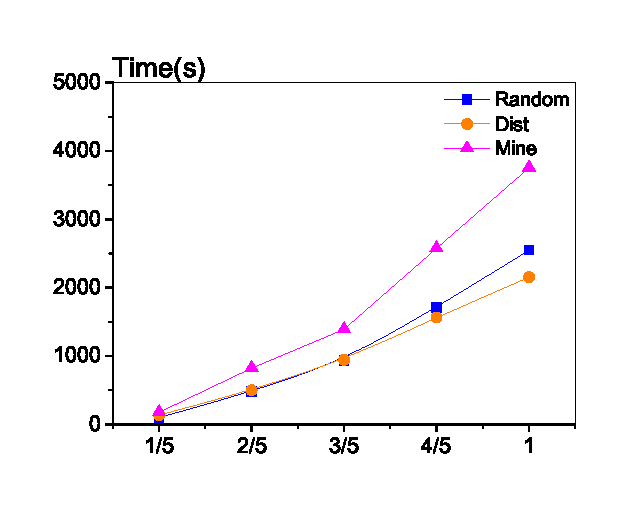
\includegraphics[width=4.7cm]{scaletimeno.eps}
%\end{minipage}%
%}
%\caption{Scale-up with Input Data ($\rho=0.7$)}\label{fig:scale}
%\end{figure}
%
%\subsubsection{Regression}\label{sec:eval:regression}
%In this part, we trace the regression behavior of $Mine$.
%We can estimate the amount of regression by comparing the number of
% \qids ever fixed with the number of distinct \qids fixed. The first number
%contains repeated \qid fixes. Because the number of \qids in a dataset can be
%extremely large especially with very long records. As such we restrict this
%experiment to datasets with cutoff = 5.
%
%Table \ref{tab:regression} shows that in all
%datasets, differences between the last two columns are very small,
%indicating that in practice, very little regression (on average about 0.13\%)
%occurred.
%
%Another interesting finding is that the number of distinct \qids fixed
%is much smaller than the number of unsafe \qids in the original data (column 2).
%On average, fixing one \qid actually causes 4.28 unsafe \qids to be sanitized.
%This validates our hypothesis that by suppressing some items to fix one \qid,
%the algorithm actually fixes other unsafe \qids at the same time as well.
%\PC{I think that we should remove this and add an experiment with varying sensitive items number}
%%?g
%%?gWe record the number of original distinct unsafe qids,
%%?gthe number of the distinct unsafe qids and the total fixed qids.
%%?gShown in Table \ref{tab:regression}, we
%%?g find that the  distinct unsafe qids really fixed is much less than the
%%?g original unsafe ones. In a conclusion, once a qid is fixed, it
%%?g may effect other correlated qids and diminish the number of
%%?g   unsafe qids dramatically.
%%?g   The average ratio is about 4.28, indicating that one fixed qid will help to fix
%%?g another 4.28 qids.
%%?g
%%?g  Another important characteristic of our algorithm is that the regression just plays a tiny role in our
%%?g algorithm.
%%?g We choose one qid in the buffer each time and fix it. The regression will work when such fixed qid will break the
%%?g previously fixed ones, thus causing the algorithm to recheck the previously fixed ones. However, according to Table \ref{tab:regression} , such
%%?g influence only accounts for a tiny part of the total fixed qids, since
%%?g The difference between distinct fixed qids and all fixed qids is very small. The average ratio of rechecking qids is only
%%?g   $0.13\%$, suggesting that one fixed qid will cause 0.13 previously fixed ones to be unsafe.
%%?g
%
%\begin{table}[th]
%\caption{Qid Fixing and Regression (\PartialR, $\rho=0.7$)}
%\centering
%\begin{tabular}{|l|r|r|r|r|r|} \hline
%Dataset 	& Orig Qids & Orig Qids &  Qids Fixed  & Qids Fixed   \\
%(cutoff=5)	&(Total)  & (Unsafe) &( Distinct)  &(All)   \\ \hline \hline
%POS  & 196968 & 111112 & 36888 & 36924\\ \hline
%WV  & 82109	&62341	&15437	&15487\\ \hline
%Retail  & 129358	&109687	&21789&	21839\\ \hline
%Syn  & 592440	&574145	&123156	&123156\\ \hline
%\end{tabular}
%\label{tab:regression}
%\end{table}
%
%\subsection{Effects of DnC Strategy}\label{sec:eval:effect}
%In this section, we analyze the effectiveness of the divide and conquer strategy on the quality
%of solution(in terms of information loss) and time performance.
%%parameters for optimization defined in our algorithm help to ameliorate the time performance by the largest extent but remain the quality of the suppressed datasets.
%%We have 4 different parameters including partial suppression policies
%%
%%\subsubsection{Partial Suppression Strategies}\label{sec:eval:partialsuppression}
%%The following experiments illustrate the result of different suppression
%%strategies. Figure \ref{sec:eval:infoloss} suggests that $Mine$ outperforms
%%the other two different strategies in information loss and association rule
%%mining (See Table \ref{tab:rules2}) but doesn't do as well in relative
%%entropy. $Dist$ outperforms the other two strategies in retaining the data
%%distribution. The log function we take on the y-axis indicates that relative
%%entropy of $Dist$ is much better than peers. Although it doesn't perform well
%%in information loss, such a disadvantage doesn't outweigh its advantage.
%%Since the occurrence of each item in the dataset remains almost the same and
%%the probability of each item can be precisely estimated. Time performances of
%%the three approaches are in the same range. We therefore conclude that the
%%performances of our two heuristics are in our expectations and such processed
%%result can be highly useful for downstream applications.
%%
%%\begin{figure}[th]
%%\centering
%%  \flushleft
%%\subfigure[ $\rho=0.7$]{\label{fig:partialrelative}
%%\hspace{-5mm}
%%\begin{minipage}[c]{0.22\textwidth}
%%\flushleft
%%  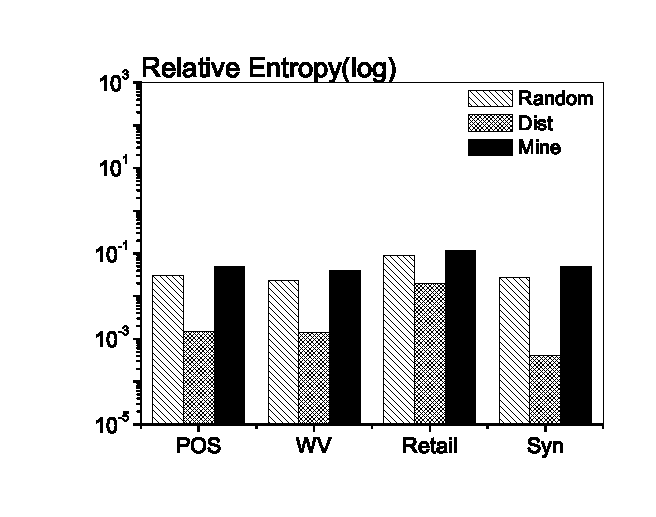
\includegraphics[width=4.9cm]{relative7ours.eps}
%%\end{minipage}%
%%}
%%\subfigure[ $\rho=0.7$]{
%%\hspace{3mm}
%%\begin{minipage}[c]{0.20\textwidth}
%%\flushleft
%%  \includegraphics[width=4.5cm]{partialtime.eps}
%%\end{minipage}%
%%}
%%\caption{Comparison among Partial Suppression Strategies}
%%\label{fig:partial}
%%%\textit{Partial(R)} suppresses sensitive only, \textit{Partial(L)} suppresses items on left side of a inference, and \textit{Partial(ALL)} suppresses items on both sides of a inference.}\label{fig:fft}
%%\end{figure}
%
%%\subsubsection{Variation of $t_{max}$}\label{sec:eval:timebound}
%We choose $Retail$ as our experimental object since $Retail$ is the most
%time-consuming datasets which can terminate within an acceptable time without DnC strategy.
%The value of $t_{max}$ determines the size of a partition in DnC. Smaller
%$t_{max}$ can give rise to more partitions. Here, we
%evaluate how partitioning helps with time performance and
%its possible effects on suppression quality.
%Figure \ref{fig:timebound-a} shows the relationship between partitions
%and information loss. The lines of $Random$ and $Dist$ are flat, indicating that
%increasing $t_{max}$ doesn't cost us the quality of the solution. $Mine$
%shows a slight descending tendency at first and then tends to be flat.
%We argue that a reasonable $t_{max}$ will not deteriorate our result quality.
%
%
%
%On the other hand, figure \ref{fig:timebound-b} shows that
%time cost increases dramatically  with the increase of  $t_{max}$.
%The reason is that  partition  decreases the cost of enumerating \qids which
%is the most time-consuming part in our algorithm. Moreover, parallel
%computing is also a major reason for acceleration.
%
%
%%This can be explained by Equation (\ref{eq:costfunc}).
%%As Figure \ref{fig:scale:b} shows,
%%the time cost for \PartialR on Retail is a slow exponential function, say
%%$\epsilon^{|T|}$ where $\epsilon$ is small. Now, if decreasing $t_{max}$ causes
%%a split of data into equal halves. The expected time cost will be
%%$2\epsilon^{\frac{|T|}{2}}$. This rough estimation clearly gives rise to
%%an exponential speed up.
%
%
%%Figure \ref{fig:timebound} shows that the time performance increases
%%exponentially with the increase of $t_{max}$.However, the quality of our result almost remains the same, which indicates that
%%partition is a reasonable method which can be applied to our algorithm.
%%The line tends to be plain when $t_{max}$ becomes larger,
%%because the expected time is less than $t_{max}$,
%% suggesting that no partitions will be executed.
%
%%timebound
%\begin{figure}[th]
%\flushleft
%\subfigure[Information Loss]{
%\label{fig:timebound-a}
%\hspace{-4mm}
%\begin{minipage}[c]{0.23\textwidth}
%\flushleft
%  \includegraphics[width=4.7cm]{timeloss.eps}
%\end{minipage}%
%}
%\subfigure[Time Performance]{
%\label{fig:timebound-b}
%\begin{minipage}[c]{0.23\textwidth}
%\flushleft
%  \includegraphics[width=4.7cm]{timetime.eps}
%\end{minipage}%
%}
%\caption{Variation of $t_{max}$ ($\rho = 0.7$)}\label{fig:timebound}
%\end{figure}
%%
%%\begin{figure}[th]
%%\flushleft
%%\subfigure[Information Loss]{
%%\hspace{-4mm}
%%\begin{minipage}[c]{0.23
%%\textwidth}
%%\flushleft
%%  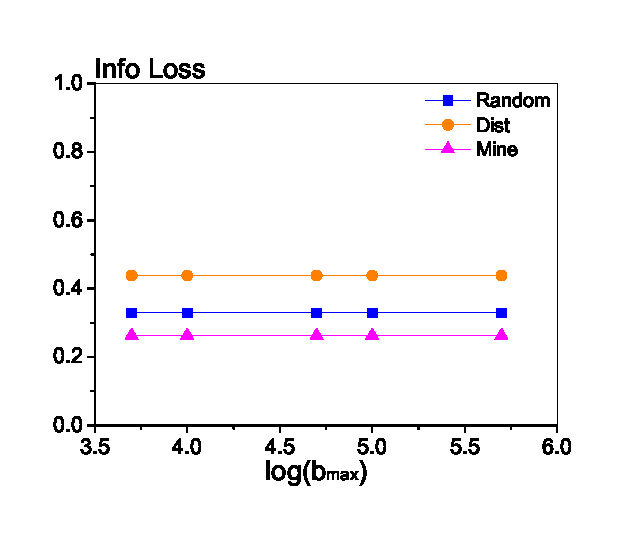
\includegraphics[width=4.7cm]{buffersizeavg.eps}
%%\end{minipage}%
%%}
%%\subfigure[Time Performance]{
%%\begin{minipage}[c]{0.23\textwidth}
%%\flushleft
%%  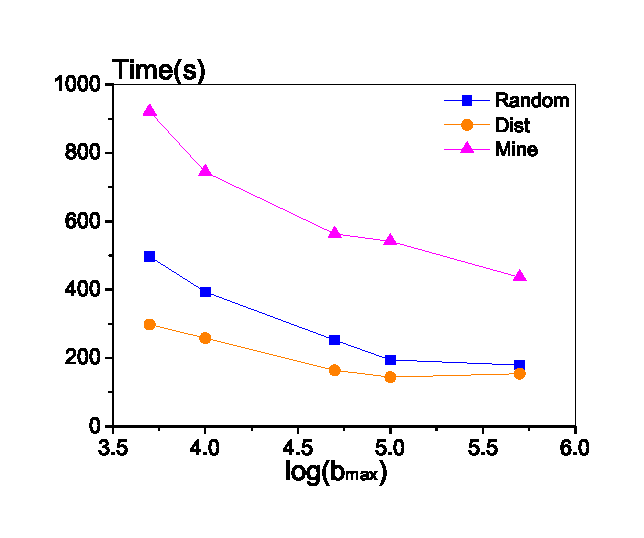
\includegraphics[width=4.7cm]{buffersize.eps}
%%\end{minipage}%
%%}
%%\caption{Variation of Buffer Size $B$ ($\rho=0.7$)}\label{fig:buffersize}
%%\end{figure}
%%
%
%%\subsubsection{Variation of $b_{max}$}\label{sec:eval:buffersize}
%%
%%This experiment (See Figure \ref{fig:buffersize}) illustrates the impact of varying $b_{max}$ on performance.
%%We choose $WV$ as our experimental object since the number of
%%distinct \qids are relatively smaller than other datasets and our algorithm
%%can terminate within an acceptable time even we set $b_{max}$   small.
%%
%%Note first that varying $b_{max}$ has no effect on the information loss which
%%indicates that this parameter is purely for performance tuning.
%%At lower values, increasing $b_{max}$ gives almost exponential
%%savings in running time. But as $b_{max}$ reaches a certain point, the speedup
%%saturates, which suggests that given the fixed size of the data,
%%when $B$ is large enough to accommodate all \qids at once after some iterations
%%, further increase in $b_{max}$ is not useful.
%%We notice that the line in $Mine$ is still descending. The reason is that
%%$Mine$ suppresses fewer items and retains more \qids, in that case the buffer is
%%not large enough to fill all \qids.
%%The other purpose of setting a reasonable value for $b_{max}$ is to limit the
%%amount of memory use.
%%
%%\subsection{A Comparison to Permutation Model}
%%In this section, we compare our algorithm with a permutation method proposed
%%in \cite{2011:TKDE:Anonymous}. We adopt the $\rho$-uncertainty privacy model
%%\cite{Cao:2010:rho} and use an randomized partial suppression algorithm to
%%satisfy it, while the method proposed in \cite{2011:TKDE:Anonymous} publishes
%%the aggregated values for the sensitive attributes,
%%thus no strong sensitive association rule exists at all
%%in the published data and thus meets our privacy requirements.
%%Here we compare the latest work of permutation technique
%%\cite{2011:TKDE:Anonymous} with ours. Permutation divides the
%%datasets into two parts: sensitive and non-sensitive and publishes the
%%aggregated values for the sensitive attributes, therefore our information
%%loss metric is not applicable there. Since the quality of their result is
%%measured by K-L divergence\cite{Lin91divergencemeasures}, we decide to
%%compare them in the quality of data distribution. We use K-L divergence as our
%%standard.(Notice that we use the symmetric form to compare with the
%%generalization method.) They guarantee that each sensitive transaction $T$
%%satisfy a privacy degree p. i.e. The probability of associating any
%%transaction $t\in T$ with a particular sensitive item $s\in D_S$ does not
%%exceed 1/p. In other words, we can set $\rho$ equals 1/p. We set $p=4, 6, 8,
%%10, r=4$ and select 10 sensitive items which are  their default values and
%%use $Gray$ as their heuristic which shows the best performance. In the
%%following experiments, we use $Gray$ to represent their algorithm.
%% We conduct experiments on $WV$ which is also their experimental
%%object to make strong and convincing comparison.
%%
%%Figure \ref{fig:permutation1} shows the result of K-L divergence.
%%All variants of our algorithm outperform $Gray$ in
%%preserving the data distribution. $Dist$ shows
%%a much better performance with an average value of $5.8 \times 10 ^{-5}$.
%%Figure \ref{fig:permutation2} shows the result of time performance.
%%Even though $Gray$ is clearly a winner, our algorithms
%%terminate within acceptable time.
%%Overall, we argue that our partial suppression methods
%%outperform the permutation method.
%%
%%\begin{figure}[th]
%%\flushleft
%%\subfigure[K-L Divergence]{\label{fig:permutation1}
%%\hspace{-4mm}
%%\begin{minipage}[c]{0.23
%%\textwidth}
%%\flushleft
%%  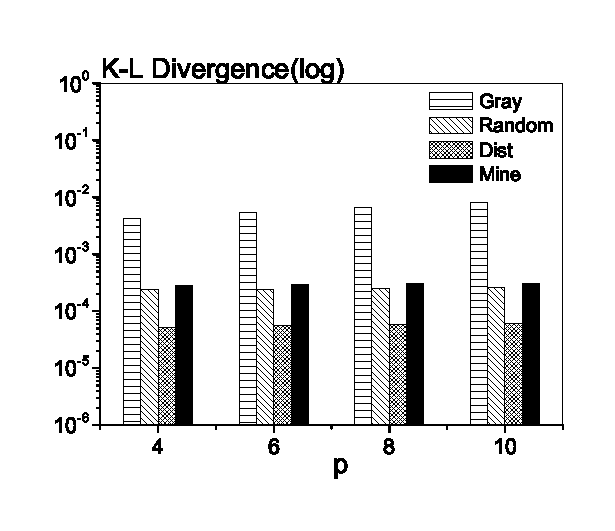
\includegraphics[width=4.7cm]{anatomy.eps}
%%\end{minipage}%
%%}
%%\subfigure[Time Performance]{\label{fig:permutation2}
%%\begin{minipage}[c]{0.23\textwidth}
%%\flushleft
%%  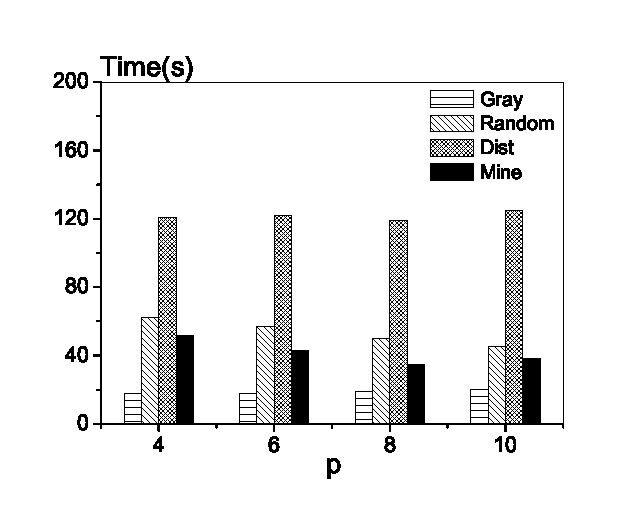
\includegraphics[width=4.7cm]{anatomytime.eps}
%%\end{minipage}%
%%}
%%\caption{Comparison with Permutation }
%%\end{figure}
%
%%exponentially with the decrease of buffer size while the Information loss remains the same.
%% The slope also tends to be zero at the end of the curve
%%because all of the qids in short records can be put in the buffer at one time,
%%thus making the function of buffer less powerful. The function of $b_{max}$ ont only ameliorates the time performance
%%.but is
%%designed for setting an upper limit of memory capacity
%%
%%\begin{figure}[th]
%%\flushleft
%%\subfigure[Information Loss]{
%%\label{fig:longrecord-a}
%%\hspace{-4mm}
%%\begin{minipage}[c]{0.23
%%\textwidth}
%%\flushleft
%%  \includegraphics[width=4.7cm]{lravgloss.eps}
%%\end{minipage}%
%%}
%%\subfigure[Time Performance]{
%%\label{fig:longrecord-b}
%%\begin{minipage}[c]{0.23\textwidth}
%%\flushleft
%%  \includegraphics[height=4.1cm,width=4.7cm]{lr.eps}
%%\end{minipage}%
%%}
%%\caption{Variation of $\lmin$ ($\rho=0.7$)}\label{fig:longrecord}
%%\end{figure}
%%
%%
%%
%%\subsubsection{Variation of $\lmin$ }\label{sec:eval:longrecord}
%%%\KZ{We may wanna do more experiments here with smaller $\lmin$. I think we
%%%will see the dip in the curve for Syn-1 and WV as well given a small enough
%%%$\lmin$.}
%%Figure \ref{fig:longrecord-a} first verifies that $\lmin$ is a performance
%%parameter which doesn't affect the solution quality much.
%%
%%The value of $\lmin$ essentially determines what portion of the data is handled
%%as short records and what port is handled as long records.
%%When $\lmin$ is small, more records are handled by \HandleLongRecord.
%%Because \HandleLongRecord involves finding intersections between \qid
%%containers, it can be increasingly expensive with the average size of
%%long records if there are more frequent itemsets in these records.
%%This is evident from the result of Retail. Thus we see the
%%curve goes up to the left.
%%Divide-and-conquer actually solves this problem to some extent.
%%If $\lmin$ is not large enough for a certain dataset,
%%$\sum_{|R| \ge \lmin}\max_{t \in R} \csize(t)$ in Equation (\ref{eq:costfunc})
%%tends to be very large, which triggers the DnC optimization.
%%
%%When $\lmin$ is large, more records are handled by \HandleShortRecords.
%%The complexity of \HandleShortRecords is largely determined by the \Enum function
%%whose cost increases with the length of the \qids. Therefore, we see to the right
%%of Retail and also in WV and Syn-1, the curves goes up. One interesting point is
%%that, for some dataset such as Retail, there exists a particular value
%%for $\lmin$ which minimizes the time cost, that is, the lowest point in the curves.
%
%
%
%
%%As $\lmin$ increases, more records are handled by \HandleShortRecords.
%%In case of Syn-1 and WV which have few records longer than 12, the total cost
%%is dominated by \HandleShortRecords which is in turn dominated by \Enum function,
%%and increases exponentially with the length of records.
%%
%%In case of Retail which comes with a lot more records longer than 12, the total
%%cost is initially dominated by \HandleLongRecord in which computing the
%%intersection of containers is the most expensive part. As we increase $\lmin$
%%and move more input records from \HandleLongRecord to \HandleShortRecords,
%%the time savings in less intersection computation outweighs the
%%additional time costs for enumerating \qids in \HandleShortRecords. As a result,
%%as $\lmin$ increases from 12 to 18, the total time cost decreases.
%%But as the number of long record diminishes, \HandleShortRecords becomes to
%%dominate the suppression process. At a certain point, additional cost in
%%enumeration of \qids outweighs the saveings in \HandleLongRecord, and the
%%total execution time starts going up.
%
%%The last experiment illustrates the importance of
%% $\lmin$ in our algorithm.
%%Generally speaking, time performance has exponent relation with $\lmin$,
%%since the number of qids increase exponentially
%%with the record length.
%%On the other hand, Retail has many more longer records, and as such we see
%%an interesting turning point in its curve.
%%To understand this strange curve, we should
%%review the function of $\lmin$ at first. We delete all
%%sensitive items in the records where the number of
%%non-sensitive items larger than to $\lmin$ to accelerate the program while on the other
%%hand we set those records whose length is larger
%%than  $\lmin$ as special cases in our
%%algorithm.
%%When $\lmin$ is small, the cost of intersection operations in \HandleLongRecord
%%may exceed the whole scanning cost.
%%Therefore, the line in retail drops at first because $\lmin$ is not large
%%enough for retail and increases dramatically when  $\lmin$ comes to 20.
%
%%\subsection{Summary}\label{sec:eval:summary}
%%Our main purpose is to keep as many items as possible. Just as the
%%optimal results in Table \ref{tab:optimal}, finding an optimal solution is
%%impossible within limited time. However, results of global suppression
%%and generalization algorithm is far from satisfactory.
%%Our algorithm outperforms them in information loss, a common metric widely used in previous work, symmetric relative entropy and the remained rules which are defined by us as two important metric of set-valued datasets.
%%To optimize our algorithm, we introduce a divide-and-conquer strategy
%%and the result shows the effectiveness of this method.
%%Although our algorithm is linear with the data size
%%, we still try to optimize our algorithm.
%%We plot figures by varying those parameters seperately.
%% All of those results show a
%%common phenomenon that the time performance becomes
%% much better but the quality almost remains the same.
%%In summary, the experiment result shows that our algorithm
%%has a much more promising application prospect than the previous work does.
%
%
%
%
%%\begin{table*}[th]
%%\centering
%%\begin{tabular}{|c|l|c|c|c|c|} \hline
%%Dataset (cutoff=5)	& Orig Qids & Orig Unsafe Qids & Distinct Qids Fixed  & All Qids Fixed   \\ \hline \hline
%%POS  & 196968 & 	111112	 & 45648	 & 45713\\ \hline
%%WV  & 82109 & 	62341	 & 19718	 & 19751\\ \hline
%%Retail  & 129358	 & 109687 & 	30065	 & 30107\\ \hline
%%Syn-1 &  187273 & 	177018 & 	46999	 & 46999\\ \hline
%%Syn-2  & 592440	 & 574145	 & 154593	 & 154593\\ \hline
%%\end{tabular}
%%\caption{Tracing Qid Fixing and Regression, set $\rho=0.7$ using Partial(L)}
%%\label{tab:datasets}
%%\end{table*}
%
%%\begin{table*}[th]
%%\centering
%%\begin{tabular}{|c|l|c|c|c|c|} \hline
%%Dataset (cutoff=5)	& Orig Qid & Orig Unsafe Qid & Distinct Qids Fixed  & All Qids Fixed   \\ \hline \hline
%%POS  &196968	&112852	&37262	&37312\\ \hline
%%WV  &129358	&110574	&21841	&21896\\ \hline
%%Syn-1 &187273	&177018&	37707	&37707\\ \hline
%%Syn-2  &592440	&574146	&123156	&123156\\ \hline
%%\end{tabular}
%%\caption{Tracing Qid Fixing and Regression, set $\rho=0.5$ using Partial\_R}
%%\label{tab:datasets}
%%\end{table*}
%
%%\begin{table*}[th]
%%\centering
%%\begin{tabular}{|c|l|c|c|c|c|} \hline
%%Dataset (cutoff=5)	& Orig Qid & Orig Unsafe Qid & Distinct Fixed Qid & Fixed Times   \\ \hline \hline
%%POS  &196968	&155860	&52039	&52410\\ \hline
%%WV  &82109	&75778	&20242&	20451\\ \hline
%%Retail & 129358	&123423&	27419&	27620\\ \hline
%%Syn-1 &187273	&177276	&42427	&42428\\ \hline
%%Syn-2 & 592440	&587439	&140814&	140814\\ \hline
%%\end{tabular}
%%\caption{Tracing Qid Fixing and Regression, set $\rho=0.3$ using Partial\_ALL}
%%\label{tab:datasets}
%%\end{table*}
%
%%\begin{table*}[th]
%%\centering
%%\begin{tabular}{|c|l|c|c|c|c|} \hline
%%Method & Info Loss & Time Cost   \\ \hline \hline
%%TDControl  && \\ \hline
%%Global  && \\ \hline
%%Partial\_R  && \\ \hline
%%\end{tabular}
%%\caption{Time cost in different Iteration}
%%\label{tab:datasets}
%%\end{table*}
